\documentclass[a4paper,12pt]{article}
\usepackage[italian]{babel}
\usepackage[utf8]{inputenc}
\usepackage{graphicx}
\usepackage{listings}
\usepackage{color}
\usepackage[usenames,dvipsnames,svgnames,table]{xcolor}

\title{Guide to RavenDAQ}
\author{Marco Baruzzo, elbaru90@gmail.com}

\begin{document}
	\maketitle

	\titlepage

	\tableofcontents
	\newpage

	\section{Installation}
		Raven Code prerequisites:
		\begin{itemize}
			\item Gigabit Ethernet board (compatible with UDP jumbo packet)
			\item LabView 2017 (or previous in compatibility mode)
			\item Linux-based OS (Theoretically it works also with Windows)
		\end{itemize}
		RavenDAQ doesn't need any other programs, if in the PC are installed LabView it will work.

		\subsection{Procedure}
		\begin{itemize}
			\item Copy the RavenDAQ folder in the PC;
			\item Disconnect the PC from the LAN or WIFI;
			\item Connect the FEC to the PC with the Ethernet cable and power in it;
			\item Open a terminal and try to ping the FEC, it will answer to the ping request ("ping 10.0.0.2");
			\item In the network option select UDP packet with jumbo frame (9000 MTU);
			\item Open ports in the firewall (UDP packets in/out for 6006, 6007, 6023, 6024, 6039, 6040, 6263, 6519, 6520);
			\item Open the SC2.vi and try to initialize the FEC to check if it is working or not (If not it will show an error).
		\end{itemize}



	\section{Settings}
		\subsection{RavenDAQ connection settings} 
			Before starting the acquisition it is important to set the right number of APV and timestamp number on the DAQ interface. The other settings normally are already correct. \\
			The millisecond 

		\subsection{Checking the mappings}
			The first things to do is check or modify the APV mapping in the specific file (\textit{apv\_mapping}).\\ 
			In the file, firstly, we find the dimensions of the APV surface in terms of PAD with row per columns logic (for example 16 PAD x 8 PAD, 16 row and 8 columns), after there is the PAD order, from top to bottom and from left to right.\\
			\begin{minipage}[c]{0.49\textwidth}
				For example this:\\
				\centering
				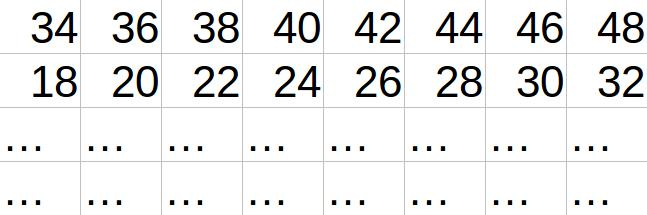
\includegraphics[scale=0.3]{mapping.png}
			\end{minipage}
			\begin{minipage}[c]{0.49\textwidth}
				\centering
				became:\\
				34\\
				36\\
				38\\
				40\\
				42\\
				44\\
				46\\
				48\\
				18\\
				20\\
				22\\
				24\\
				26\\
				28\\
				30\\
				32\\
				...\\
			\end{minipage}
		
 	\section{Decoding raw file}
 		DATE saves data from FEC in real time, so it's important to understand how the date are stored in the raw file.\\
 		This is only a little preview on how complicated it is:\\
 		\vspace{0.2cm}\\
 		{\scriptsize
 		\begin{minipage}[c]{0.49\textwidth}
			\texttt{0000 0080 0000 0000 0000 0000 0000 0000\\
			0000 0000 0100 0000 ffff ffff 646b db58\\
			2782 0e00 cc19 0100 1600 0000 0100 0000\\
			0000 0000 0000 0000 0000 0000 0400 0000\\
			008f 0e6b {\color{lime}00}{\color{blue}43 4441} {\color{pink}a00f bbaa} {\color{red}0bfb 0b68\\
			0c59 0c58 0c57 0c56 0c56 0c55 0c54 0c56\\
			0c54 0c54 0c53 0c55 0c55 0c53 0c54 0c54\\
			0c54 0c56 0c54 0c51 0c54 0c54 0c53 0c53\\
			0c54 0c53 0c55 0c54 0c54 0c55 0c55 0c55\\
			0b67} {\color{green}04a6} {\color{red}0c57 0bfb 0c5a 0c58 0c54 0c56\\
			0c56 0c55 0c54 0c55 0c52 0c54 0c53 0c53\\
			0c55 0c55 0c54 0c52 0c53 0c55 0c54 0c54\\
			0c54 0c55 0c56 0c54 0c54 0c54 0c54 0c54\\
			0c54 0c53} {\color{green}04a4} {\color{red}0c54 0bf9 0b66 0c59 0c5a\\
			0c56 0c59 0c55 0c55 0c53 0c54 0c53 0c55\\
			0c53 0c52 0c50 0c52 0c50 0c50 0c51 0c50\\
			...\\
			0c54 0c54 0c54 0c54 0c54 0c52 0c53 0c56\\
			0c53 0c53 0c54 0c53 0c54 0c55} \colorbox{darkgray}{\color{green}04a4} {\color{red}0c54}\\
			\colorbox{darkgray}{{\color{green}0384 03e0 0456} {\color{red}0b11} {\color{green}0390 03ee 0394 0392}}\\
			\colorbox{darkgray}{\color{green}0399 0398} {\color{yellow}09c4} \colorbox{darkgray}{\color{green}0398} {\color{yellow}0a40 0a52 0a7c 0a24\\
			0a44 0a50 0a6c 0a1c 0a3b 0a60 0a80 0a05\\
			0a3b 0a5b 0a75 09ef 0a36 0a77 0a7f 0a2b\\
			0a43 0a61 0a65 0a16 0a45 0a5e 0a69 0a0a\\
			0a36 0a63 0a72 09f4 0a4c 0a7e 0a79 0a25\\
			0a5a 0a70 0a7c 0a25 0a3f 0a4e 0a78 0a12\\
			0a2c 0a4d 0a69 0a04 0a36 0a58 0a89 0a24\\
			0a3c 0a64 0a78 0a28 0a38 0a58 0a61 0a0f}\\}
		\end{minipage}
		{\scriptsize
		\begin{minipage}[c]{0.49\textwidth}
			Here we some colors:
			\begin{itemize}
				\item {\color{lime} the number ot the apv}
				\item {\color{blue} mean ADC in ASCII, from here there are the data from the APV}
				\item {\color{pink} other bit value from FEC}
				\item {\color{red} 0 digital values ($>$3000)}
				\item {\color{green} 1 digital values ($<$1200)}
				\item {\color{yellow} analogical values (1200$<$ and $<$3000)}
				\item \colorbox{darkgray}{\color{white} show the 12 word part with mean the start}\\
				\colorbox{darkgray}{\color{white}of the analog value from PADs AVP for the first timestamp}
			\end{itemize}
		\end{minipage}}
 	

\end{document}